\pagebreak 
 \begin{UseCase}{CUA02}{Actualizar estado}{Un analista modificará el estado del proceso de la cosntancia o boleta}
	\UCitem{Version}{1.0}
  \UCitem{Actor}{Analista}
  \UCitem{Propósito}{El analista informa por vía internet al estudiante o egresado el progreso de su documento para que  evite ir físicamente a las oficinas de gestión escolar.}
  \UCitem{Entradas}{
    \begin{itemize}
    \item Botón de cambio de estado.
	\item Los estados del documento son: 
	\end{itemize}
			\begin{itemize}
				\item Solicitado
				\item En proceso
				\item Finalizado
				\item Entregado
			\end{itemize}
  }
  \UCitem{Origen}{
    \begin{itemize}
    \item Documentos solicitados obtenidos desde el repositorio de datos.
      \end{itemize}
  }
  \UCitem{Salidas}{
    \begin{itemize}
		\item Mensaje de información {\bf AlertaDocumentoFinalizado}
    \end{itemize}
  }
  \UCitem{Destino}{
    \begin{itemize}
      \item Pantalla.
    \end{itemize}
  }
  \UCitem{Precondiciones}{
   \begin{itemize}
      \item El alumno debió haber solicitado un documento al sistema.
      \item El analista debió haber sido identificado por el sistema.
      \item El documento  todavia no esta en el estado de finalizado.
    \end{itemize}
  }
  \UCitem{Postcondiciones}{
    \begin{itemize}
      \item Se modifica el estado del documento en el sistema.
    \end{itemize}
  }
  \UCitem{Observaciones}{
		\begin{itemize}
			\item El analista podrá modificar de manera secuencial los estados del documento.
		\end{itemize}
  }
  \UCitem{Errores}{
  	\begin{itemize}
  	\item Ninguno.
  	\end{itemize}
	}
  \UCitem{Tipo de ejecución}{Secundaria, viene de CUG02 Iniciar Sesión Empleado}
	\UCitem{Volatilidad}{Baja}
	\UCitem{Madurez}{Alta}
	\UCitem{Prioridad}{Alta}
  \UCitem{Estado}{Autorizado}
	\UCitem{Autor}{Alberto Maldonado Romo}
	\UCitem{Revisor}{Juan Antonio Guzman Chavez }
\end{UseCase}

\begin{UCtrayectoria}{Principal}
  \UCpaso[\UCactor] Edita el estado del documento  haciendo click en la opción del menú ``Actualizar estado”.
  \UCpaso Muestra la pantalla  {\bf UIActualizarEstado}
  \UCpaso[\UCactor] Indica los diferentes  tipos de estado del documento haciendo click sobre una opción del select.
  \UCpaso[\UCactor] Da click en el botón\IUbutton{Modificar Estado} 
  \UCpaso  Válida que sse finalizo el documento. [TAA] 
\end{UCtrayectoria} 

\begin{UCtrayectoriaA}{A}{Peticiones excedidas} 
\UCpaso Muestra el mensaje {\bf AlertaDocumentoFinalizadon}
  \UCpaso Notificará al estudiante o egresado por medio de un correo electrónico. 	
\end{UCtrayectoriaA}

\textsc{\begin{figure}[!htbp]
    \centering
        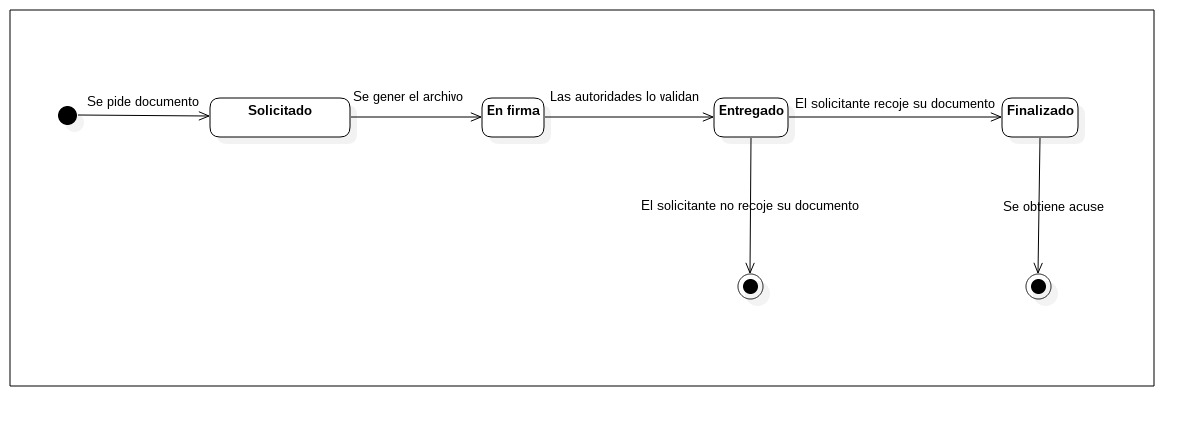
\includegraphics[width=0.6\textwidth]{images/UI/Analista/diagramEst}
    \caption{Diagrama de estados}\end{figure}}
\FloatBarrier
%-------------------------------------- TERMINA descripción del caso de uso.


